\documentclass[12pt, a4paper]{article}


\usepackage{amsmath}
\usepackage{wasysym}
\usepackage{amsthm}
\usepackage{amssymb}
\usepackage[utf8]{inputenc}
\usepackage[dutch]{babel}
\usepackage{graphicx}
\usepackage{float}
\usepackage{subfig}
\usepackage[a4paper, left=1in]{geometry}
\usepackage{xcolor}
\usepackage{booktabs} % Top and bottom rules for tables
\usepackage{hyperref}
\hypersetup{urlcolor={blue}, colorlinks=false, linkcolor=., citecolor=.}
\usepackage[backend=biber,style=authortitle-comp]{biblatex}
\addbibresource{minicursus2018.bib}
\usepackage{csquotes}

% prutsen met fonts, xelatex compiler nodig!
%\newcommand{\mainfont}{[HumorSans.ttf]}
%\usepackage{mathspec} %loads fontspec as well
%\setmainfont{\mainfont}
%\setmathrm{\mainfont}
%\setmathfont(Digits,Latin){\mainfont}

\newcommand{\du}{\,\mathrm{d}}
\newcommand{\bgtan}{\mathrm{\,Bgtan\,}}
\newcommand{\bgsin}{\mathrm{\,Bgsin\,}}
\newcommand{\bgcos}{\mathrm{\,Bgcos\,}}
\newcommand{\p}{\mathcal{P}}
\newcommand{\R}{\mathbb{R}}
\newcommand{\Z}{\mathbb{Z}}
\newcommand{\N}{\mathbb{N}}
\newcommand{\q}{\mathbb{Q}}
\newcommand{\BO}{\mathcal{O}}

\theoremstyle{definition}
\newtheorem{oef}{Oefening}[subsection]

\title{Practicum differentiaalvergelijkingen: De Lorenz Attractor}
\author{Pieter Luyten}
\date{November 2018}

\begin{document}

\maketitle

\begin{figure}[H]
    \centering
    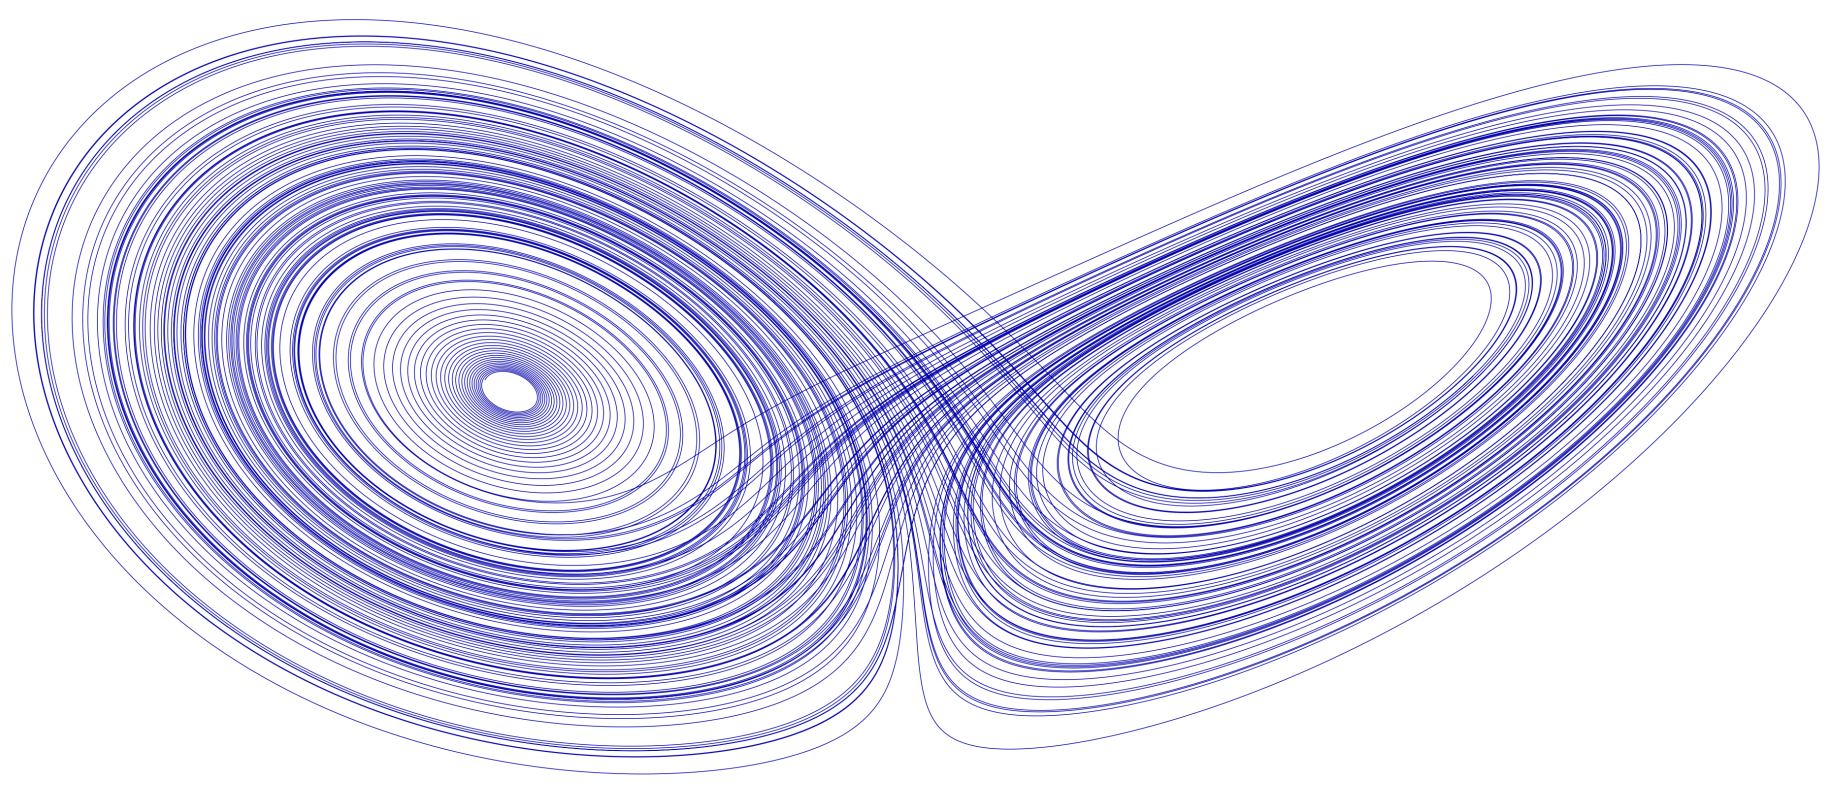
\includegraphics[width=0.9\linewidth]{header_verslag.png}
\end{figure}

\section{Inleiding}
In dit practicum bestuderen we het gedrag van de Lorenz attractor voor een specifieke set parameters. De Lorenz attractor is een stelsel van 3 differentiaalvergelijkingen:
\begin{align}
    x'(t) &= -\sigma x + \sigma x \nonumber \\
    y'(t) &= r x -y -xz\\
    \label{eq: stelses lorenz}
    z'(t) &= -bx +xy \nonumber
\end{align}
Hierin zijn $\sigma, r, b$ 3 parameters. We stellen voor de rest van dit document deze gelijk aan:
$$\sigma = 10 \qquad r=28 \qquad b = 8/3$$
Deze differentiaalvergelijking werd bestudeerd met numerieke methoden. Ik heb IJulia notebooks gebruikt voor de numerieke methoden om de vergelijking op te lossen en verdere analyse. Voor de analyse van de kritieke punten heb ik het package sympy gebruikt om met symbolische vergelijkingen te werken. De gebruikte code kan je \href{https://nbviewer.jupyter.org/github/Cubedsheep/practicum-diff-Julia/blob/master/practicum%20-%20Julia.ipynb?fbclid=IwAR0w5uD6396VRiiF5jM1AxzXG7EB4HG5WAsDRnNsDRpx_s_2yaZP3bjLWWA}{hier
} vinden.



\section{Kritieke punten}
We berekenen eerst de kritieke punten van het systeem van differentiaalvergelijkingen. Dit zijn punten waarin elke afgeleide gelijk is aan 0. In dit geval zijn er 3 kritieke punten: de oorsprong ($O$), een punt met negatieve $x$-coördinaat ($A$) en een punt met positieve $x$-coördinaat. De coördinaten van de kritieke punten zijn:
\begin{align*}
    O &= (0, 0, 0)\\
    A &= (-8.485, -8.485, 27.0)\\
    B &= (8.485, 8.485, 27.0)
\end{align*}
Voor de analyse van de kritieke punten bepalen we de eigenwaarden en bijhorende eigenvectoren van de Jacobiaan in deze punten. Dit geeft:
\begin{align*}
    A: \lambda_1 &= -13.85, \Vec{v_1} = \left[ \begin{array}{cc}0.85 \\ -0.32 \\ 0.39\end{array} \right] \lambda_2 = 0.0939 + 10.1945i, \Vec{v_2} = \left[ \begin{array}{c} -0.26-0.29i \\ 0.032-0.56i \\ 0.719 \end{array} \right]\\
    \lambda_3 &= 0.0939 - 10.1945i, \Vec{v_2} = \left[ \begin{array}{c} -0.26+0.29i \\ 0.032+0.56i \\ 0.719 \end{array} \right]\\
    B: \lambda_1 &= -13.85, \Vec{v_1} = \left[ \begin{array}{cc}0.85 \\ -0.32 \\ -0.39\end{array} \right] \lambda_2 = 0.0939 + 10.1945i, \Vec{v_2} = \left[ \begin{array}{c} -0.26-0.29i \\ 0.032-0.56i \\ -0.719 \end{array} \right]\\
    \lambda_3 &= 0.0939 - 10.1945i, \Vec{v_2} = \left[ \begin{array}{c} -0.26+0.29i \\ 0.032+0.56i \\ -0.719 \end{array} \right]\\
    O: \lambda_1 &= -22.827, \Vec{v_1} = \left[\begin{array}{c} -0.614\\  0.788\\ 0\end{array} \right] \lambda_2 = 11.827, \Vec{v_2} = \left[ \begin{array}{c} -0.416\\-0.909\\0\end{array}\right]
    \lambda_3 = \frac{8}{3}, \Vec{v_3} = \left[ \begin{array}{c}0\\0\\1\end{array} \right]
\end{align*}
Bij de punten $A$ en $B$ zien we dat er 1 negatieve en 2 complexe eigenwaarden zijn. De eigenwaarde $\lambda_1$ is negatief, de oplossingen zullen dus naar het vlak door A en loodrecht op $\Vec{v_1}$ getrokken worden. In dit vlak hebben we een spiraalpunt, de 2 andere eigenwaarden zijn namelijk complex. Dit is een onstabiel spiraalpunt want de reële delen van $\lambda_2$ en $\lambda_3$ zijn positief.\\
\\
In het punt $O$ zijn er 3 reële eigenwaarden, 1 negatief en 2 positief, de component van de richtingsvector volgens $\Vec{v_1}$ zal dus negatief zijn en de oplossingen naar een vlak loodrecht op $\Vec{v_1}$ door $O$ trekken. In dit vlak hebben we een onechte bron, de oplossingen bewegen weg van $O$ in dit punt.



\section{Periodische oplossingen}
Hoewel het gedrag van de oplossingen van vergelijking \ref{eq: stelses lorenz} in het algemeen chaotisch is, zijn er oplossingen met specifieke beginvoorwaarden die een periodiek gedrag vertonen. Dit periodiek gedrag duiden we aan met een sequentie van A's en B's die zegt hoe vaak en in welke volgorde de oplossing rond elk punt draait.

\subsection{Oplossing AB}
Voor de beginvoorwaarde $\textbf{x}(0)$:
$$x(0) =−13,763 610 682 134, \quad y(0) =−19,578 751 942 452, \quad   z(0) = 27$$
vinden we een periodieke oplossing AB. Deze draait dus een keer rond A, een keer rond B en komt dan terug op de beginwaarde uit. Deze beginwaarde kunnen we gebruiken om de nauwkeurigheid van numerieke methodes te testen. We benaderen met 3 numerieke methodes, de methode van Euler, de verbeterde methode van Euler en Runge-Kutta van orde 4, de periodieke oplossing en zoeken de stapgrootte die nodig is om de fout op de eindwaarde kleiner dan $10^{-5}$ te krijgen.\\
\\
De functies om de oplossing numeriek te benaderen geven als return value een lijst met opeenvolgende punten van de oplossing. In deze lijst zoeken we het punt dat het dichtst bij de beginwaarde ligt, noem dit punt $D$, het punt ervoor $C$ en het punt na $D$ noemen we $E$. Deze afstand is echter niet altijd de dichtste afstand tot de beginwaarde, hiervoor moeten we de afstand van de beginwaarde tot de lijnstukken $[CD]$ en $[DE]$. Als deze afstand kleiner is, en de loodrechte projectie van de beginwaarde op dit lijnstuk ligt, is dit de kleinste afstand tot de beginwaarde. Als de 2 loodrechte projecties niet op het lijnstuk liggen, gebruiken we de tijd tot het dichtste punt als benadering van de periode. In het andere geval projecteren we $\textbf{x}(0)$ op het lijnstuk waar het het dichtste bij ligt, noem deze projectie $P$. We berekenen dan de verhouding $\frac{|DP|}{|CD|}$ of $\frac{|DP|}{|DE|}$. Dit vermenigvuldigen we met de stapgrootte $h$ en tellen we op bij de tijd tot het punt $D$ om een schatting voor de periode $T$ van de periodische baan te krijgen.\\
Deze methode geeft volgende waardes voor $h$ en $T$ zodat $|\textbf{x}(0) - \textbf{x}(T)| < 10^{-5}$

\begin{figure}[H]
    \centering
    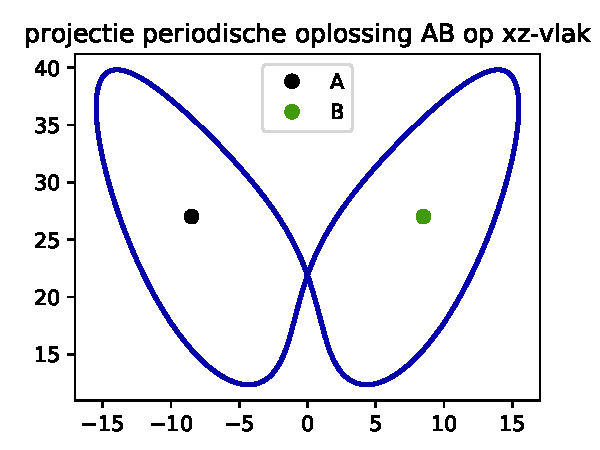
\includegraphics[width=0.5\linewidth]{projectie_opdracht_3.pdf}
    \caption{De projectie in het xz-vlak van een periodische oplossing AB}
    \label{fig: AB}
\end{figure}

\subsection{Oplossing AAAB}
Er is gegeven dat voor de beginwaarden
$$x(0) =−11, 998 523 280 062, \quad y(0) \in [-16, -15] \quad   z(0) = 27$$
er een periodische oplossing is van de vorm AAAB. Het gedrag van de oplossingen is chaotisch maar we kunnen wel de continuïteit in de beginvoorwaarde gebruiken (UITWERKEN!). Als we 2 beginvoorwaarden dicht bij elkaar nemen, zullen ook de oplossingen van de differentiaalvergelijking dicht bij elkaar liggen

\begin{figure}[h]
    \centering
    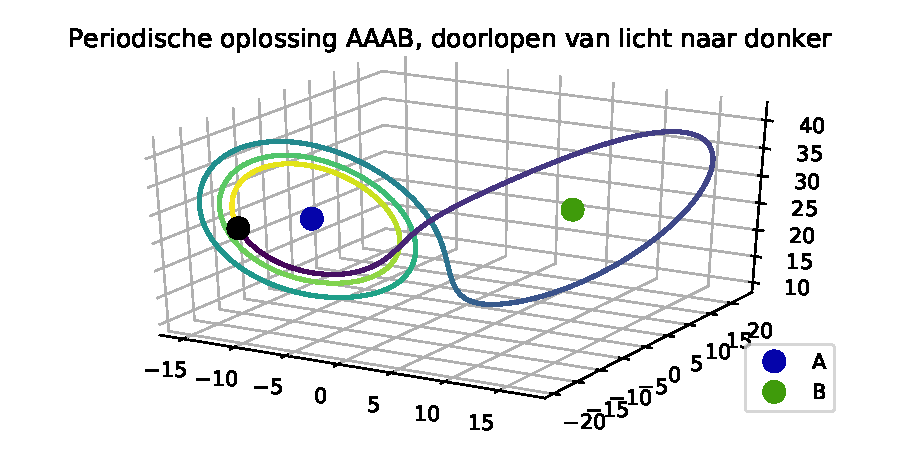
\includegraphics[width=0.9\linewidth]{periodische_baan_AAAB_opdracht4.pdf}
    \caption{Plot van een periodische baan AAAB. De kromme wordt doorlopen van geel naar paars (licht naar donker)}
    \label{fig: AAAB}
\end{figure}

\begin{figure}[h]
    \centering
    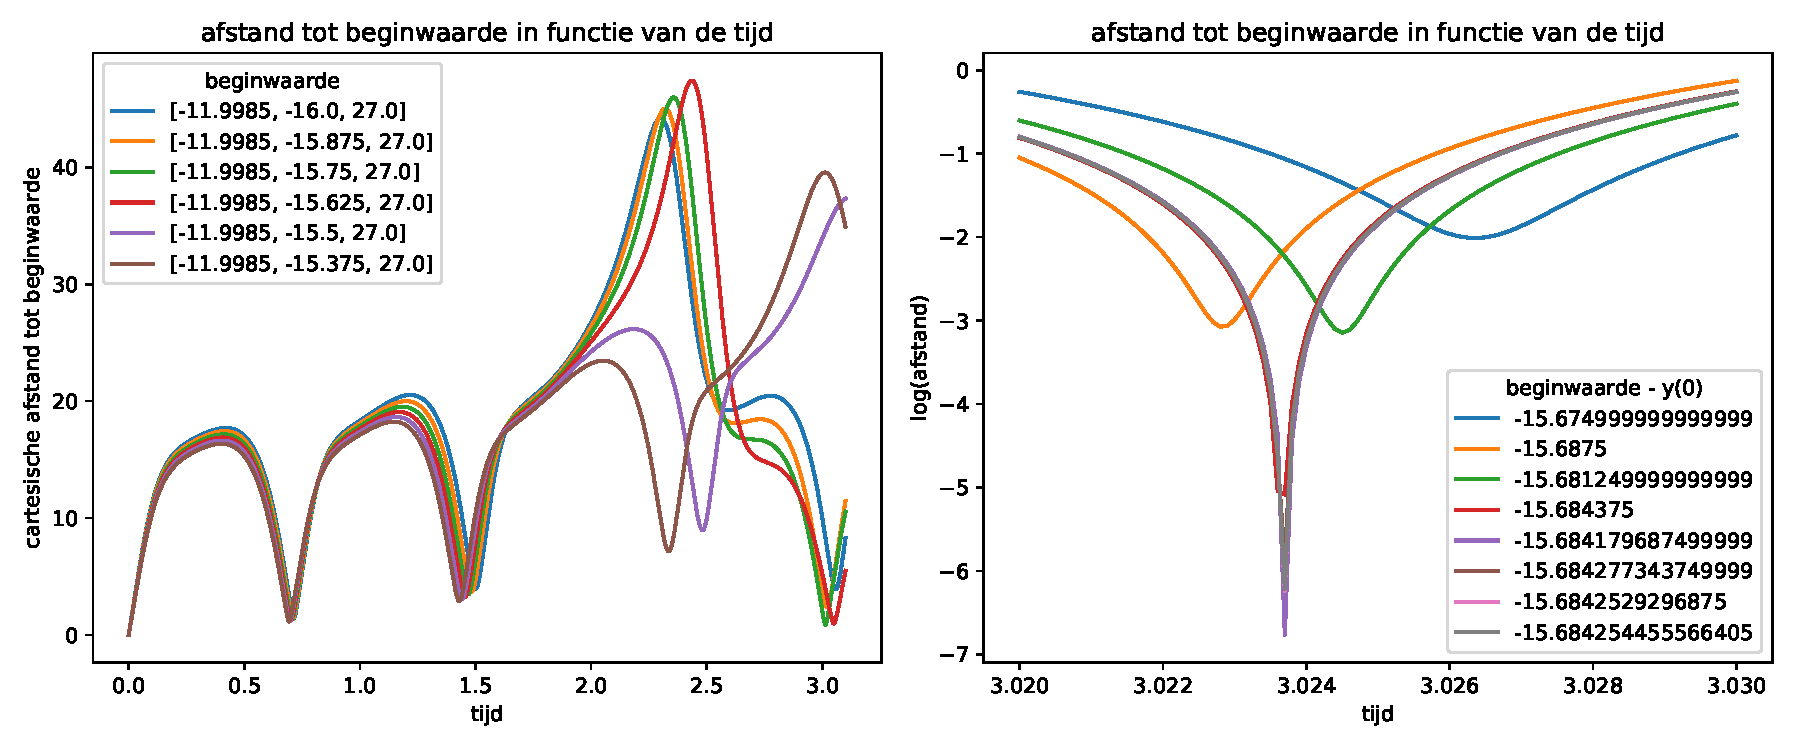
\includegraphics[width=\linewidth]{afstand_beginwaarde_opdracht4.pdf}
    \caption{Links: afstand tot de beginwaarde in functie van de tijd voor een aantal beginwaarden met $y(0) \in [-16, -15]$. Rechts: de afstand tot de beginwaarde in functie van de tijd, rond het tijdstip waarop de oplossing het dichtst komt voor opeenvolgende iteraties van de verfijningsmethode}
    \label{fig: afstand}
\end{figure}

\begin{figure}
    \centering
    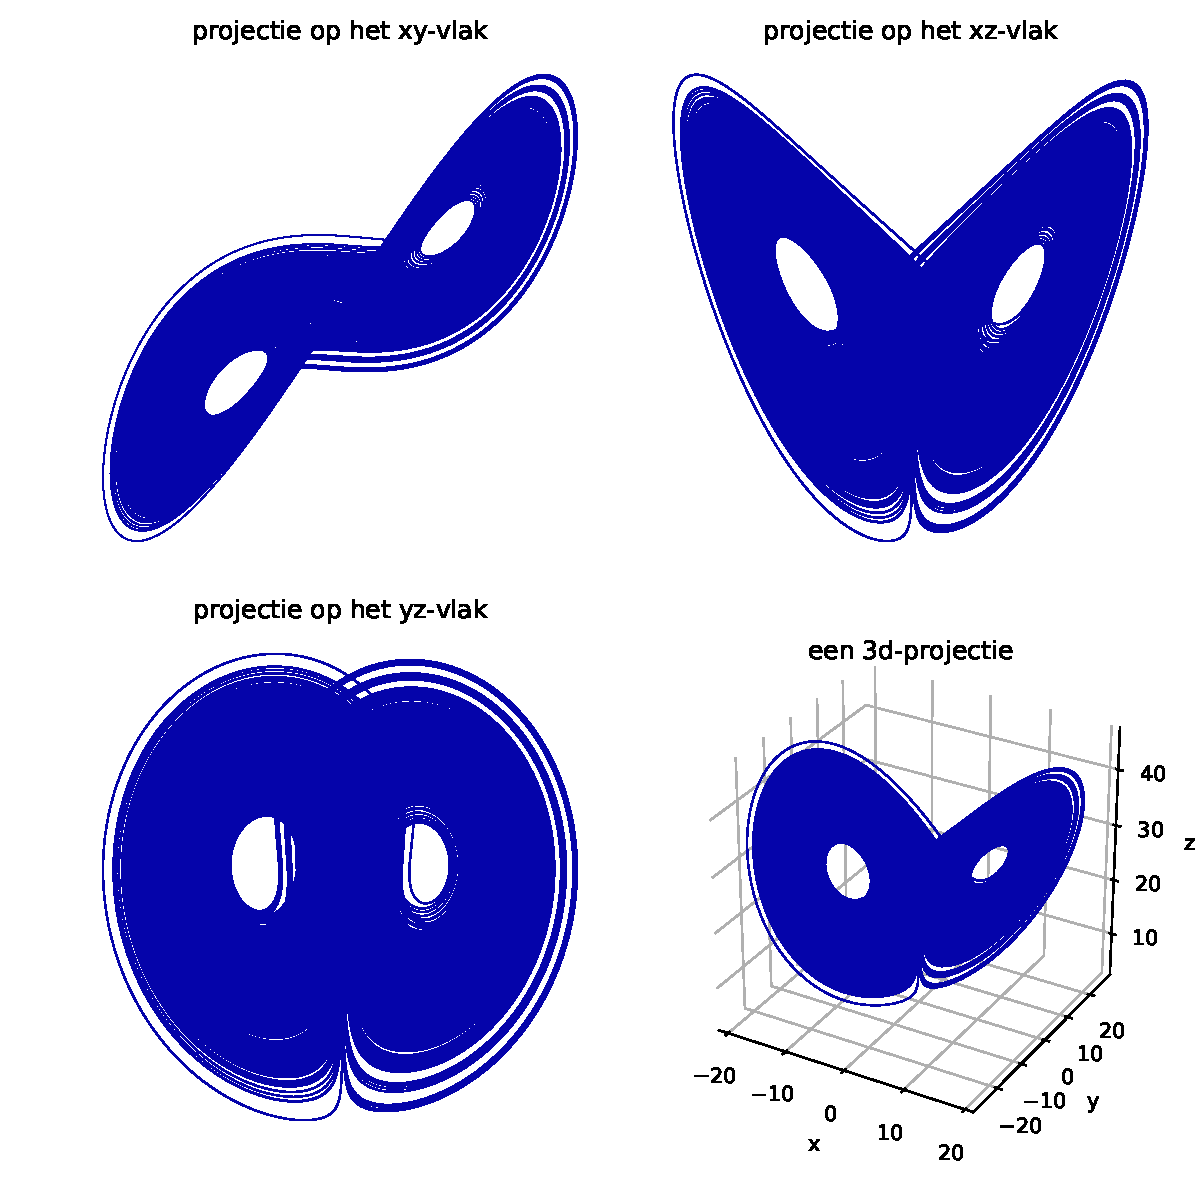
\includegraphics[width=0.9\linewidth]{projecties_opdracht_5.pdf}
    \caption{Projecties van een pad op de Lorenz attractor voor $T \rightarrow \infty$}
    \label{fig: projecties}
\end{figure}

\end{document}
